\documentclass[11pt,a4paper]{article}
\usepackage[margin=1.95cm]{geometry}
\usepackage[T1]{fontenc}
\usepackage{lmodern}
\usepackage{microtype}
\usepackage{amsmath,amssymb,booktabs,graphicx,subcaption,xcolor,hyperref}
\usepackage{enumitem}
\usepackage{float}
\usepackage{natbib}
\hypersetup{colorlinks=true,urlcolor=blue!55!black,citecolor=blue!55!black,linkcolor=blue!55!black}
\setlength{\parskip}{3pt}
\setlength{\parindent}{0pt}
\setlist{nosep,leftmargin=*}
\renewcommand{\arraystretch}{1.10}
\title{\vspace{-1.2cm}\bfseries When Is Re-evaluation Worth the Budget?\\\large Bayesian Optimisation versus CMA-ES under Noisy Observations}
\author{Alagammai Lavanya Muthiah\\Student number: A0282879E\\\small DSA4212 Final Project}
\date{November 2026}
\begin{document}
\maketitle
\vspace{-0.5cm}
\begin{center}\small\textbf{Code, configurations and numerical results:} \url{https://github.com/LavanyaMuthiah/DSA4212-BO-vs-CMAES}\end{center}
\vspace{-0.15cm}
\begin{abstract}\noindent
When observations are noisy, the lowest measured objective value need not identify the best solution. The study investigates how a fixed budget should be divided between searching new points and re-evaluating promising candidates, and whether the answer differs between Gaussian-process Bayesian optimisation (BO) and covariance matrix adaptation evolution strategy (CMA-ES). Across four five-dimensional benchmarks, two primary noise levels, three validation allocations and 20 paired seeds, no allocation is uniformly best. On noisy Rosenbrock, validation can substantially reduce selection error; on noisy Rastrigin, sacrificing search evaluations usually hurts. Follow-up studies distinguish candidate discovery from noisy ranking, test CMA-ES population size, and examine a diversity-aware shortlist and intermediate noise. The findings illustrate that the value of replication depends on landscape, noise and search quality, not merely on the optimiser's label.
\end{abstract}
\vspace{-0.15cm}
\section{Question, motivation and prior work}
Optimising a robot controller, laboratory process or machine-learning configuration may require a costly physical trial, simulation or training run for every candidate. Measurements may vary between trials even at the same setting. For example, repeating a promising chemistry experiment could confirm a genuine improvement, but consumes resources that might instead test a different setting. The decision matters when the final deliverable is one recommended configuration rather than the best-looking measurement. These are motivations, not applications directly tested here; the experiments use synthetic benchmarks to isolate the mechanisms.

Consider minimising an unknown $f(x)$ when each paid evaluation returns $y(x)=f(x)+\epsilon$, with independent $\epsilon\sim\mathcal N(0,\sigma^2)$. An unusually low observation may reflect a favourable noise draw rather than a genuinely good point. Spending calls on replication improves estimates of existing candidates but leaves fewer calls to discover new ones. The research question is therefore: \emph{under a common budget, when does end-of-run validation improve the true quality of the final recommendation, and does the answer differ between BO and CMA-ES?}

BO uses a probabilistic surrogate to balance exploration and exploitation; it is particularly attractive when objective calls are expensive \citep{jones1998,shahriari2016,frazier2018}. As discussed in the course lectures, Gaussian processes represent predictive mean and uncertainty, and a lower confidence bound (LCB) can prefer either promising or uncertain regions. BO \emph{can handle} noisy observations, including through an explicit observation-noise model, but this does not make it immune to noise: a low measured value may still be a lucky error, and the acquisition policy need not yield a reliable final recommendation. The noise model is independent, additive, zero-mean, homoskedastic Gaussian noise with a known standard deviation; it does not represent input-dependent, biased, heavy-tailed or correlated measurement errors. CMA-ES instead updates a sampling distribution using candidate rankings and learned covariance geometry, often offering much cheaper internal computation per call \citep{hansen2016}. Neither automatically solves the \emph{final selection} problem under noise. Replication versus exploration is central to stochastic simulation design \citep{binois2019}; sequential kriging-based optimisation and noisy evolutionary strategies also study noise-aware decisions \citep{huang2006,dinu2024}. The study does \emph{not} implement those papers' adaptive policies: it deliberately tests a simpler, controlled, end-of-search allocation. Following black-box benchmarking principles, the comparison uses objective-call budgets and reports computational overhead separately \citep{coco2021}.

\section{Experimental design and audited implementation}
\subsection{Exploratory development rather than a fixed recipe}
The investigation began with a 60-call BO--CMA-ES pilot, then examined CMA-ES convergence up to 1,000 calls and GP fitting cost. A weak early BO result prompted an investigation of its acquisition optimisation rather than a conclusion that BO was intrinsically inferior. In Experiment 5, improving BO reduced \emph{noise-free Sphere} mean regret at 200 calls from 1.291 to about 0.00006 across three seeds, while increasing mean CPU runtime from roughly 1.11 to 18.79 seconds in the archived pilot CSV. This is an exploratory implementation comparison, not evidence of a universal algorithm ranking. Experiments 3--6 then exposed noisy recommendation errors and the need to account explicitly for both search and repeated measurements. In 6A--6D, small-seed budget, validation and shortlist-size probes revealed instability; this motivated a 20-seed primary study, diagnostic decomposition and later sensitivity checks. Failed ideas and corrected implementations were retained as exploratory history rather than silently treating them as independent confirmatory results.

\subsection{Problems and noise}
Sphere (smooth convex), Ackley (a broad basin with oscillations), Rosenbrock (a narrow curved valley) and Rastrigin (many local minima) are minimised on $[-5,5]^5$. Their global optimum values are $f^*=0$ on this domain. For each function, the noise standard deviation is $\sigma=\eta S_f$, where $S_f$ is an independently computed objective-value interquartile-range reference scale: Sphere 23.121, Ackley 1.978, Rosenbrock 50,776.291 and Rastrigin 31.850. The primary study uses $\eta\in\{0,0.05\}$; this scale choice makes noise relative to each landscape's value distribution, rather than imposing one incomparable absolute $\sigma$.

\subsection{Search implementations}
Both methods start from the same 10 seeded design locations, and their evaluations count toward the budget. BO uses a scikit-learn Gaussian process with a Mat\'ern-$5/2$ kernel, min--max-scaled inputs to $[0,1]$ and standardised outputs and observation-noise variance supplied from the known synthetic noise setting. Kernel parameters are refitted initially and every 25 evaluations; the next point minimises a lower-confidence-bound acquisition $\mu(x)-2s(x)$ over 1,024 random proposals followed by bounded L-BFGS-B refinement. Thus the final BO implementation is \emph{not} expected improvement and does \emph{not} learn the noise variance: these details matter for reproducibility. CMA-ES uses the \texttt{cma} package, initial step size 2, population 8, box bounds and restarts on stopping; it starts at the best noisy initial design point. Both methods receive the same initial observations, although they exploit them differently. The BO policy was improved after an exploratory pilot; this tuning asymmetry is disclosed, and CMA-ES population size is tested separately.

\subsection{Budget and recommendation}
Each policy has exactly $B=600$ noisy objective calls. For validation fraction $v\in\{0,0.10,0.25\}$, the search receives $(1-v)B=600,540,450$ calls and the remaining $0,60,150$ calls re-measure a shortlist of $K=5$ lowest \emph{noisy} search observations. Repeat calls are distributed cyclically across the five candidates, including their original observations in each sample mean; the candidate with the smallest average is recommended. Retaining the initially favourable noisy observation may leave some winner's-curse bias even after remeasurement. The primary analysis fixes $K=5$ (a separate exploratory analysis examined $K=10$). The same saved maximum-budget search trajectory supplies shorter search prefixes, avoiding needless re-optimisation; each policy's accounting still charges only its own prefix and repeats. Search and validation noise are generated from separate reproducible streams.

\subsection{Scoring and uncertainty}
Only \emph{after} a recommendation is made is the known noise-free benchmark used to calculate simple regret $r=f(\hat x)-f^*$. Let $r_{\rm oracle}$ denote the minimum true regret among that policy's searched points, and $r_{\rm short}$ the minimum among its shortlist. Then
\begin{equation}\label{eq:decomp}
 r-r_{\rm oracle}=\underbrace{(r_{\rm short}-r_{\rm oracle})}_{\text{shortlist loss}}+\underbrace{(r-r_{\rm short})}_{\text{ranking loss}}.
\end{equation}
These oracle values are \emph{diagnostics}, never information available to either optimiser or selection policy. The primary study uses 20 paired seeds per primary condition and paired bootstrap intervals for each validation policy minus $v=0$ within the same method and landscape \citep{efron1993}. Intervals are exploratory and unadjusted for multiple comparisons. All 320 main search trajectories (4 functions $\times$ 2 methods $\times$ 2 noise levels $\times$ 20 seeds) and budget checks completed. These trajectories were reused to evaluate three validation fractions, with $K=5$ primary; a $K=10$ sensitivity output is saved separately. Independent cross-environment checks reproduced the tested CMA-ES policies to numerical precision, but BO search trajectories varied with BLAS floating-point behaviour despite fixed seeds; the broad findings, rather than exact per-seed BO outputs, are the appropriate target for cross-platform comparison. The packaged repository's saved-result consistency script and three smoke tests passed; they check arithmetic, budgets and selected cross-experiment matches, but are not an independent full rerun. The main experiments used Colab CPUs, with Python/library versions recorded in the configuration; the repository smoke tests ran separately in Python 3.12.

\section{Main results: no universal validation fraction}
\begin{figure}[t]
\centering
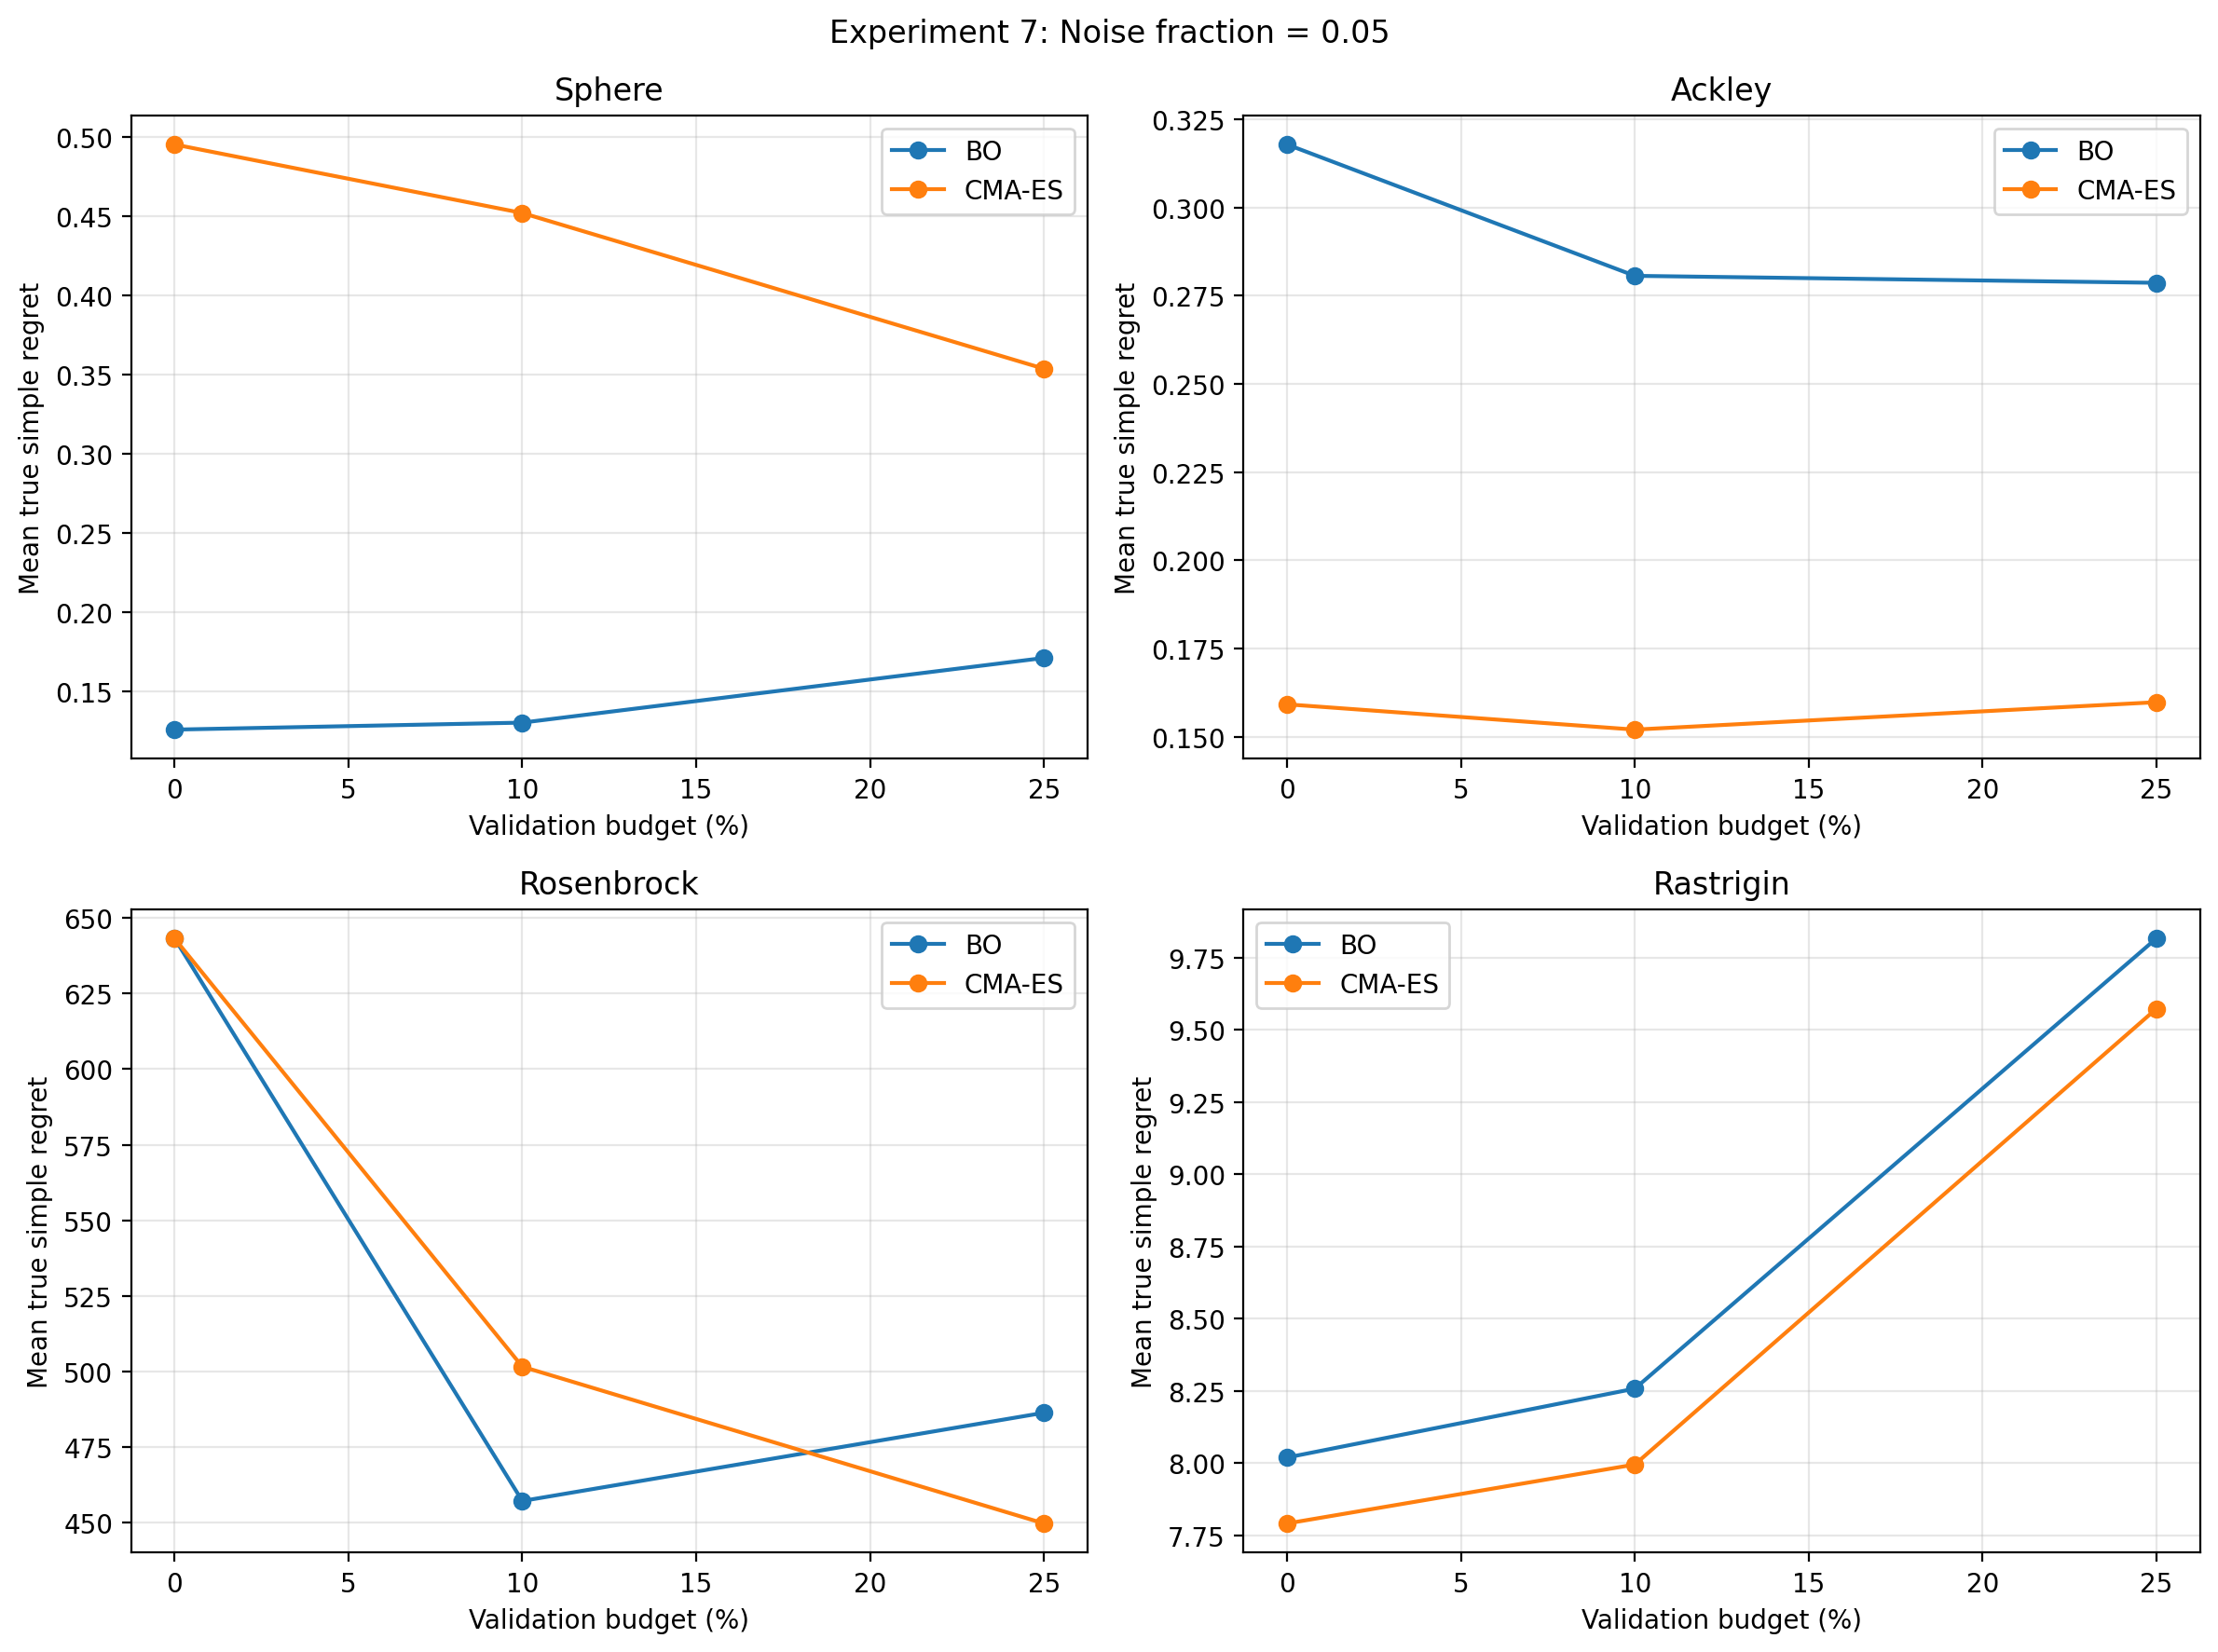
\includegraphics[width=0.94\linewidth]{figures/main_regret_noise_0.05.png}
\caption{Experiment 7, 5\% IQR noise: mean noise-free simple regret across 20 seeds versus fraction of the 600-call budget spent on end-of-run validation (lower is better). The four panels use separate vertical scales.}
\label{fig:main}
\end{figure}

Table~\ref{tab:main} isolates the noisy case. On \textbf{Rosenbrock}, BO mean regret falls from 643.28 with no validation to 457.13 at 10\% (paired change $-186.15$, 95\% bootstrap interval $[-350.14,-33.37]$). CMA-ES falls from 643.23 to 449.69 at 25\% ($-193.54$, interval $[-351.92,-55.51]$). By contrast, at 25\% on \textbf{Rastrigin}, BO worsens from 8.02 to 9.82 (paired $+1.80$, interval $[0.62,3.19]$), and CMA-ES worsens from 7.79 to 9.57 (paired $+1.78$, interval $[0.81,2.88]$). For \textbf{Sphere}, BO is already more accurate than default CMA-ES under noise and validation tends not to help BO; for \textbf{Ackley}, BO benefits modestly while CMA-ES changes little. For Rosenbrock BO, the original 25\% comparison also favoured validation numerically ($-156.97$), but its paired interval $[-341.74,17.95]$ included zero. These are within-method allocation comparisons, not formal tests of BO versus CMA-ES superiority.

\begin{table}[t]
\centering\small
\caption{Experiment 7: mean true regret at 5\% IQR noise (20 seeds). Bold is the smallest observed mean within each function--method row; selection after inspecting the same data is descriptive.}
\label{tab:main}
\begin{tabular}{llrrr}\toprule
Function & Method & $v=0$ & $v=0.10$ & $v=0.25$\\\midrule
Sphere & BO & \textbf{0.126} & 0.130 & 0.171\\
 & CMA-ES & 0.495 & 0.452 & \textbf{0.354}\\
Ackley & BO & 0.318 & 0.281 & \textbf{0.279}\\
 & CMA-ES & 0.159 & \textbf{0.152} & 0.160\\
Rosenbrock & BO & 643.281 & \textbf{457.133} & 486.313\\
 & CMA-ES & 643.229 & 501.558 & \textbf{449.689}\\
Rastrigin & BO & \textbf{8.020} & 8.258 & 9.816\\
 & CMA-ES & \textbf{7.791} & 7.995 & 9.573\\\bottomrule
\end{tabular}
\end{table}

\textbf{Why does this happen?} Equation~\eqref{eq:decomp} reveals that on noisy Rosenbrock the main difficulty is not solely finding promising points: BO's mean oracle regret is 64.88 at $v=0$, versus 643.28 for its actually selected point. Its 578.40 selection gap falls to 391.25 at 10\% validation, while the oracle changes little (65.88). For CMA-ES the analogous gap drops from 566.58 to 370.29 at 25\%. At 5\% IQR noise, Rosenbrock has $\sigma\approx2{,}539$ while the median best-found regret among the 20 BO runs without validation is approximately 41; the best searched candidate was absent from the top-five noisy shortlist in all 120 noisy Rosenbrock policies ($K=5$). These comparisons illustrate severe ranking and shortlist difficulties: validation can improve the ranking of shortlisted points, but cannot recover an excluded candidate. Thus repeated measurements help distinguish noisy candidates already encountered. On Rastrigin, however, the oracle regret for BO rises from 7.61 to 9.80 as search calls are removed, while its selection gap was only 0.41 to begin with: replication cannot compensate for weaker exploration. This tests the proposed explanation for the contrasting behaviour: \emph{replicate when recommendation error is the bottleneck; continue searching when candidate discovery is the bottleneck}. The decomposition is an accounting identity, not by itself proof that a specific optimiser mechanism caused the gap. Moreover, the fraction $v$ changes both search length and selection, so the observed differences describe the entire policy, not an isolated effect of remeasurement.

\textbf{What should be used, and when?} Within this fixed-budget, five-dimensional benchmark, the choice depends on the \emph{bottleneck} and the available compute. On noisy Sphere, improved BO with no validation gave mean regret 0.126 versus 0.495 for default CMA-ES; its more accurate recommendation justifies the GP overhead only when objective evaluations are themselves expensive enough. On noisy Ackley, default CMA-ES with 10\% validation (0.152) outperformed the tested BO configurations (best 0.279), although the across-method difference was not subjected to a paired significance test. On noisy Rosenbrock, both default methods were nearly tied without validation (643.28 versus 643.23); in the original saved runs BO had its lowest mean regret at 10\% (457.13) and default CMA-ES at 25\% (449.69). An independent BO rerun on a different BLAS configuration instead favoured 25\%, so the particular best BO fraction is not robust across tested environments. Yet the later population-size check lowered CMA-ES's Rosenbrock regret to 226.70 at population 16 and 25\% validation, showing that configuration matters more than a simple method label. On noisy Rastrigin, neither method benefited from spending 25\% on validation; at $v=0$, BO and default CMA-ES were similar (8.02 and 7.79). Thus \emph{use additional validation when noise mainly corrupts the ranking of already-discovered candidates}, as the large Rosenbrock oracle--selection gap suggests; \emph{preserve search evaluations when finding good basins is harder than selecting among them}, as on Rastrigin. This is a diagnosis from controlled synthetic experiments, not a universal deployment rule. In real expensive evaluations, BO's modelling cost may be acceptable; for cheap objectives, CMA-ES's lower CPU overhead is an important advantage. The study cannot identify a universally best algorithm or allocation without testing other dimensions, noise models and tuning choices.

In the \emph{noise-free} controls, repeated measurements add no new information, and shorter search prefixes cannot improve the best encountered value. Under the tested selection rule, regret is non-decreasing with $v$ by construction; this is a sanity check of the accounting rather than independent evidence for the proposed mechanism. Importantly, \emph{zero selection gap does not mean zero optimisation regret}: the best searched point may still be far from the global optimum.

\section{Follow-up experiments prompted by the results}
\subsection{Intermediate noise (Experiment 8C)}
To test whether the 5\% condition was unusually extreme, Rosenbrock and Rastrigin were evaluated at 1\% IQR noise with 10 new seeds and the same 600-call policies. On Rosenbrock, BO drops from 185.39 at $v=0$ to 98.69 at 10\% (paired difference $-86.70$, interval $[-165.27,-12.34]$). On Rastrigin, CMA-ES instead rises from 5.77 to 10.38 at 25\% (paired $+4.60$, interval $[2.52,6.75]$). The qualitative landscape contrast therefore persists at intermediate noise. Because 8C uses new seeds, comparisons \emph{between} 1\% and 5\% noise are not paired; only allocations \emph{within} 8C are paired.

\subsection{CMA-ES population sensitivity (corrected Experiment 8A-R)}
Only population size was varied $\lambda\in\{4,8,16\}$ using the same 20 seeds. At 5\% noise and $v=0$, Rosenbrock mean regret changes from 843.68 ($\lambda=4$) to 643.23 ($\lambda=8$) and 297.42 ($\lambda=16$). In contrast, Rastrigin is best at $\lambda=8$: 11.88, 7.79 and 10.88, respectively. Larger populations can stabilise noisy rankings and explore more widely, but also yield fewer generations at a fixed evaluation budget; this is a plausible mechanism, not a proven causal explanation. Crucially, all 480 policy records for $\lambda=8$ reproduce the main Experiment 7 CMA-ES results numerically. The original 8A implementation was superseded because it did not match the main study's CMA-ES policy sufficiently for a clean sensitivity comparison. The corrected version preserves the Experiment 7 default ($\lambda=8$) and varies population size alone; all 480 \emph{search trajectories} were generated for the 4 $\times$ 2 $\times$ 3 $\times$ 20 design, and its default-policy results reproduce the corresponding Experiment 7 rows. The correction is part of the research record, not a second independent confirmation.

\begin{figure}[t]
\centering
\begin{minipage}{0.57\linewidth}
\centering\textbf{(a) CMA-ES population sensitivity}\par\smallskip
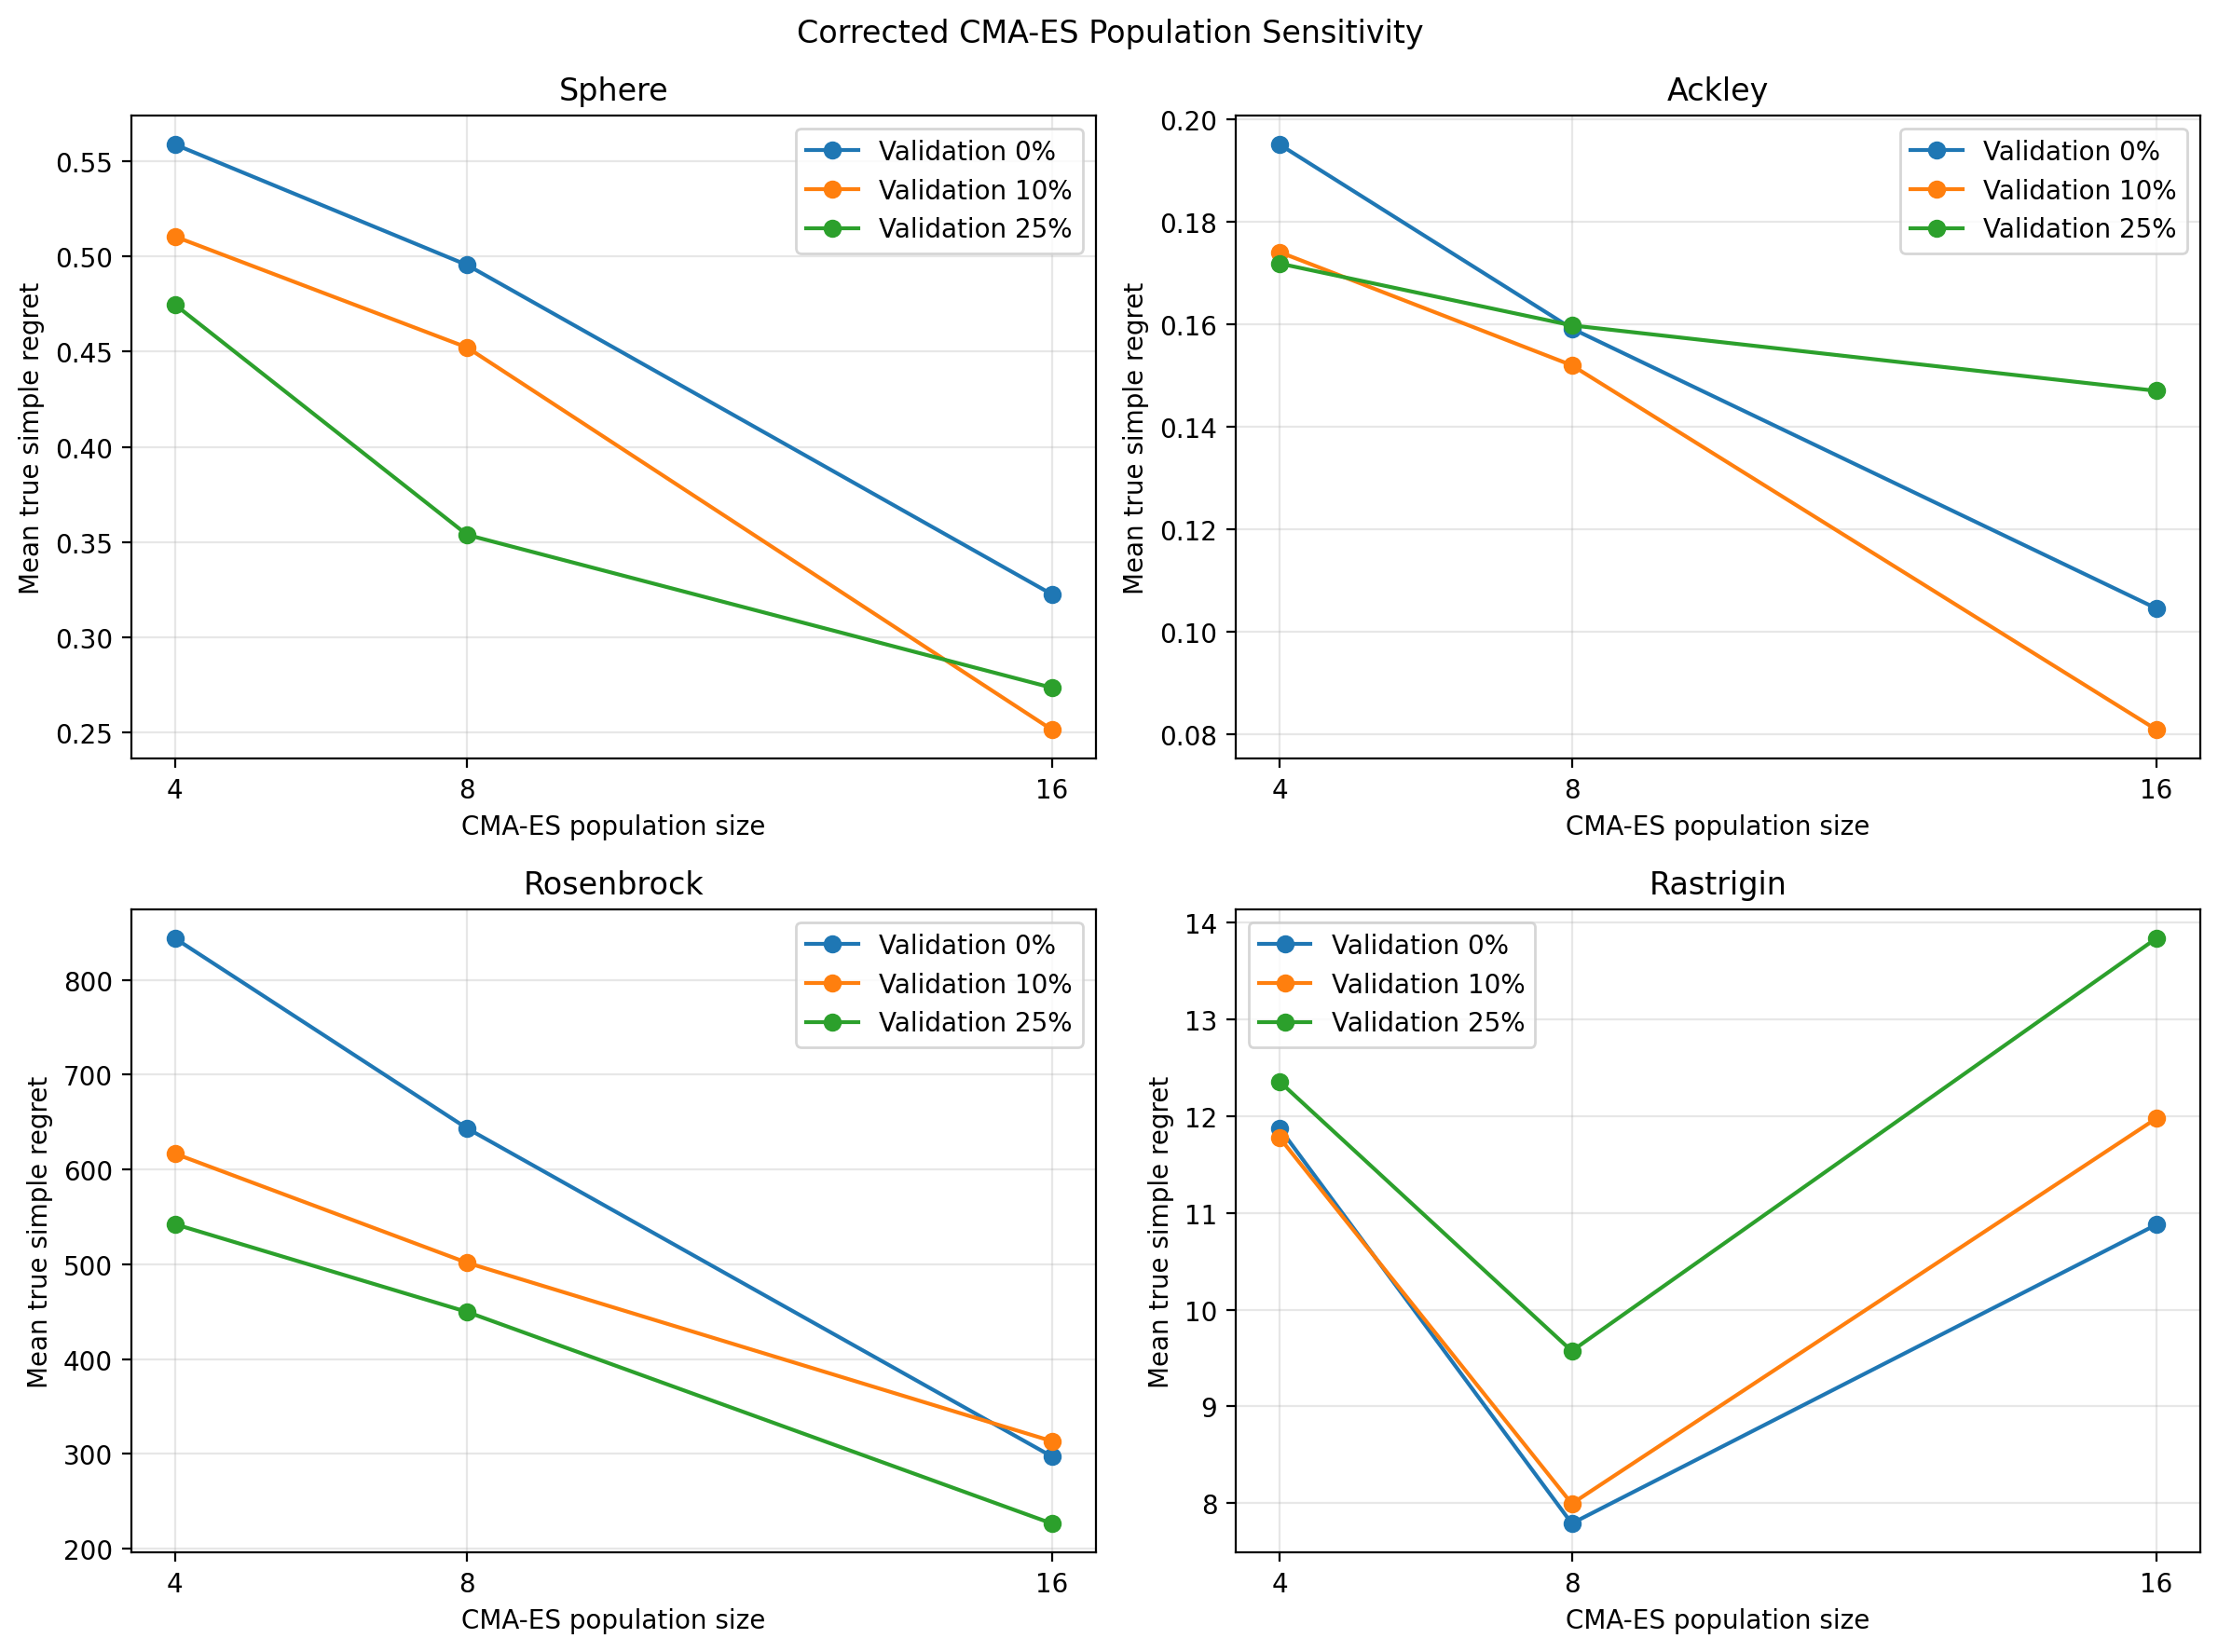
\includegraphics[width=\linewidth]{figures/population_sensitivity.png}
\end{minipage}\par\medskip
\begin{minipage}{0.57\linewidth}
\centering\textbf{(b) Intermediate noise sensitivity}\par\smallskip
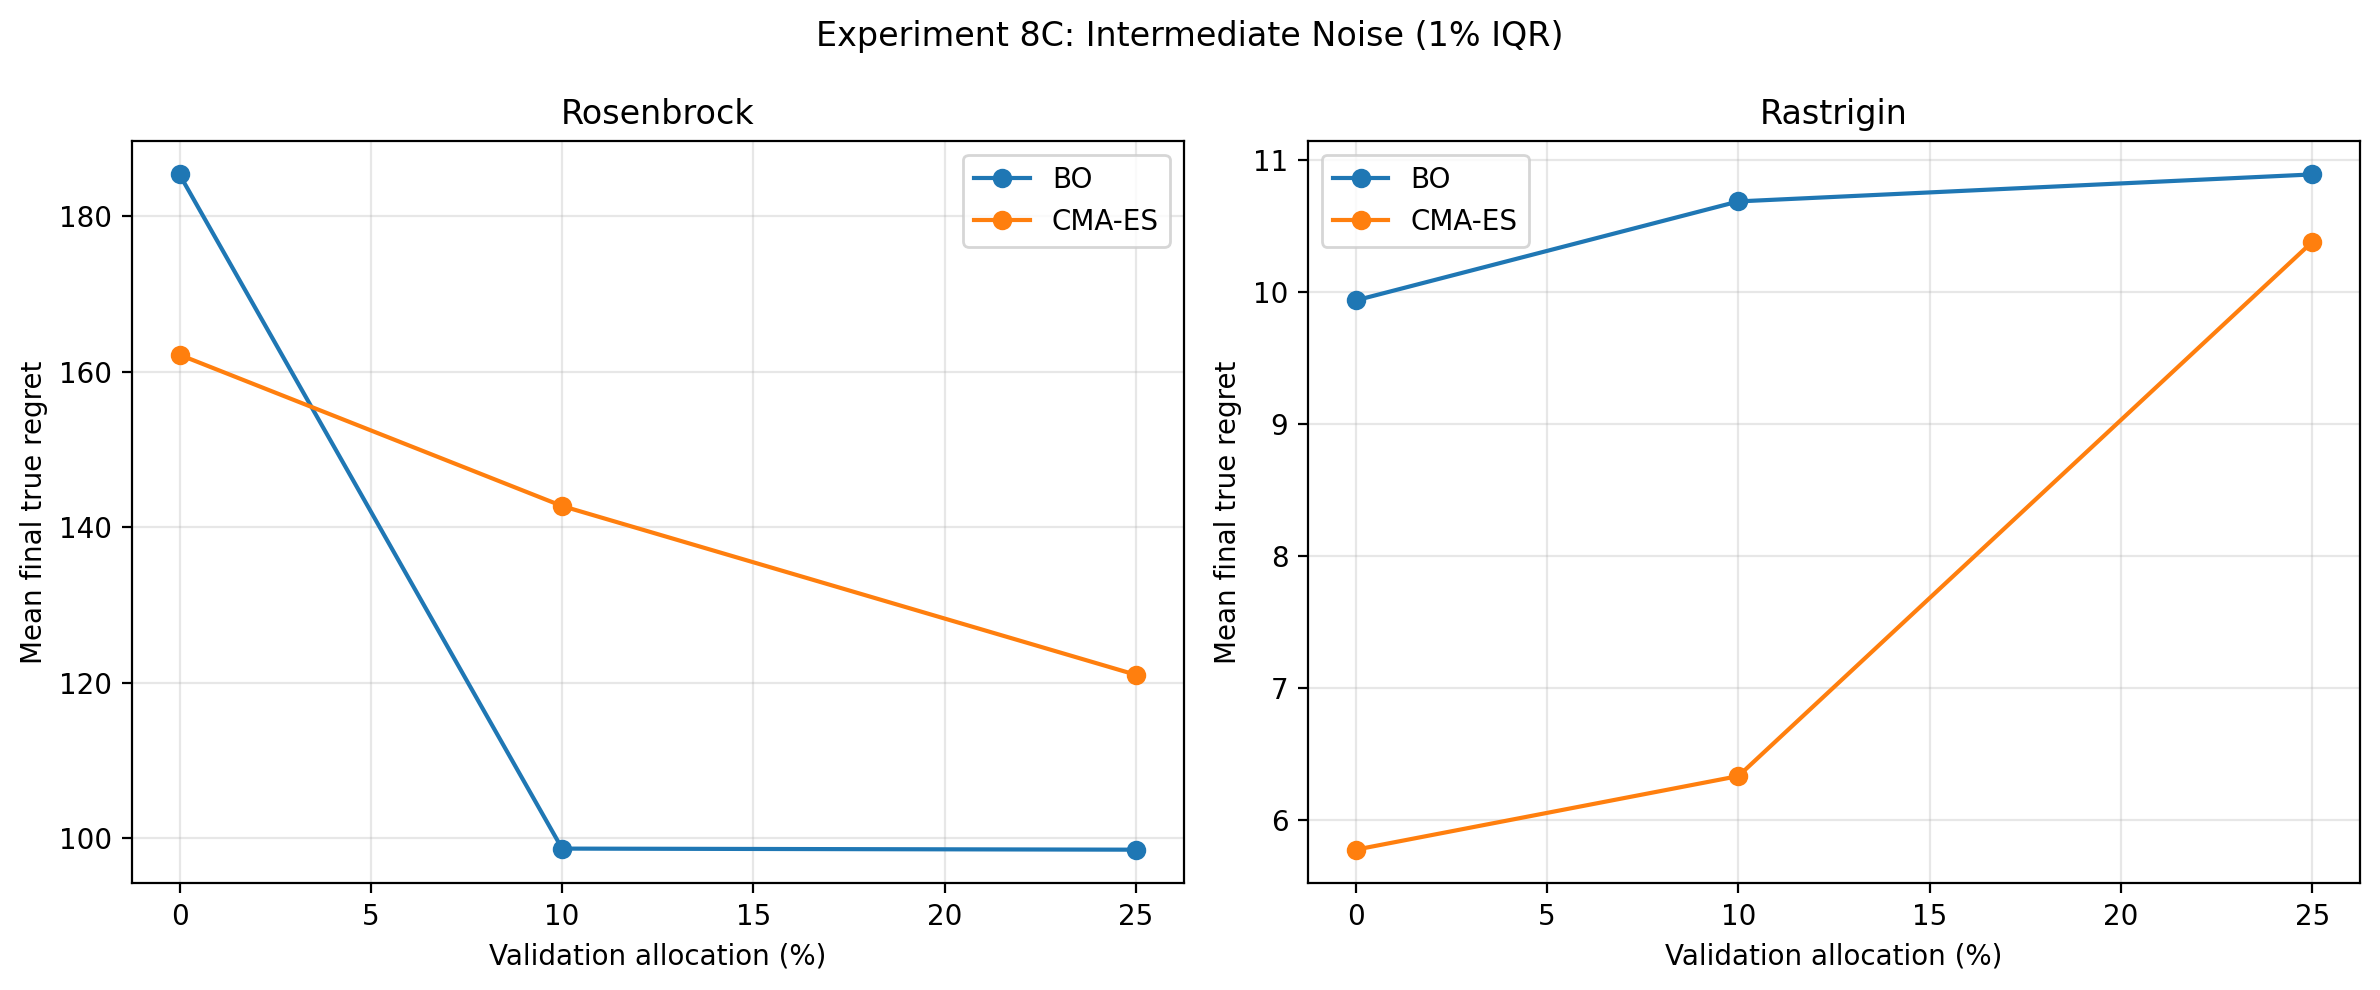
\includegraphics[width=\linewidth]{figures/noise_sensitivity.png}
\end{minipage}
\caption{Targeted checks. Top: corrected CMA-ES population-size sensitivity (5\% noise). Bottom: intermediate 1\% noise on Rosenbrock and Rastrigin. Both panels show mean noise-free simple regret (lower is better). The two panels depict different experiments and must not be compared as matched samples.}
\label{fig:followups}
\end{figure}

\subsection{Shortlist diversity (corrected Experiment 8B-R)}
The follow-up tested whether choosing spatially separated validation candidates (minimum normalised distance 0.15) would reduce shortlist loss compared with simply taking the five lowest noisy values. On Rastrigin, the BO shortlists and outcomes were identical for both policies; on noisy Rosenbrock at 10\% validation, BO's diverse shortlist improved mean regret by 50.94, but the paired 95\% interval for \emph{diverse minus top-noisy} was $[-172.24,44.26]$. All eight intervals across the two functions, two methods and two fractions included zero; for BO on Rastrigin, two comparisons were trivially zero because the shortlists were identical across all 40 policies. For BO on Rosenbrock at 10\%, only four of 20 seeds produced different shortlists. Hence the experiment found \emph{no consistent evidence} that this simple diversity constraint improves final selection. This is informative: extra spatial coverage is not enough if it excludes candidates with good true values or if the subsequent ranking remains noisy. The corrected top-noisy baseline reproduces all 160 matching Experiment 7 policies; the original 8B used a different independent validation-noise stream, which permitted within-8B comparisons but not exact reproduction of Experiment 7. The validation-noise stream was aligned to strengthen the audit trail, not because a fresh noise stream is inherently invalid.

\section{Trade-offs, limitations and conclusions}
The evidence suggests a practical decision rule, not a universal winner. \emph{When objective calls are costly and the landscape allows promising points to be found but noisy selection is unreliable} (the Rosenbrock case), reserving some calls for replication can improve the delivered answer. \emph{When discovering the right basin is the dominant challenge} (the Rastrigin case), more exploration is preferable. BO's surrogate can be attractive when evaluations are expensive; CMA-ES's cheap internal updates and covariance adaptation are attractive when evaluations are inexpensive or when local geometry is exploitable. These statements are conditional on the tested implementations and landscapes, not claims of universal superiority.

\subsection{Insights from unsuccessful attempts}
The initial BO baseline was not an adequate basis for claiming CMA-ES superiority; stronger acquisition optimisation improved quality but cost CPU time. Early two- and three-seed validation curves were unstable, so the main experiment was expanded to 20 seeds. A plausible diversity constraint did not reliably help. Finally, the corrected CMA-ES sensitivity check changed the interpretation of algorithm rankings: default settings were not universally competitive. These observations prompted follow-up experiments rather than post-hoc selection of only favourable results.

There are four main limitations. First, the benchmark suite comprises only four synthetic, five-dimensional functions with additive homoskedastic Gaussian noise; real systems may have unknown, input-dependent or non-Gaussian noise. Second, validation occurs only at the end; adaptive replication and exploration strategies may allocate calls more effectively. \citet{binois2019} study this trade-off for surrogate prediction accuracy rather than the final optimisation recommendation used here. Third, BO was improved during exploratory work, whereas CMA-ES received only a targeted population-size check, so the comparison is not between exhaustively tuned algorithms. Fourth, equal evaluation counts are \emph{not} equal CPU time: BO repeatedly fits and optimises a GP, whereas CMA-ES updates are far cheaper on these synthetic objectives. Across Experiment 7, the mean recorded runtime for a full 600-call search trajectory was 162.29 seconds for BO versus 0.13 seconds for CMA-ES on Colab CPUs (\texttt{search\_full\_runtime}); these are search times, not matched total-policy runtimes. These synthetic-objective timings should not be extrapolated directly to expensive real-world evaluations. The use of a known noise scale by BO is an additional advantage unavailable in some applications. The IQR scaling equalises a global objective-value reference, \emph{not} local signal-to-noise ratio; therefore the noise difficulty is not identical across landscapes. The study has not tested higher dimensions, multiple restart strategies for BO, unknown noise, alternative acquisition functions, or adaptive replication. The primary uncertainty intervals compare allocations within a method and do not establish statistically significant superiority of BO over CMA-ES. The small exploratory studies should not be overinterpreted. The original Experiment 7 raw \texttt{.npz} trajectories are not included in the repository: they can be regenerated from the notebook, but the corrected 8B-R downstream analysis requires those trajectories, and exact BO regeneration across BLAS environments is not assured. The trajectory-manifest hashes identify the original archived files, not necessarily regenerated files containing runtime metadata. The Experiment 5 pilot statistics are supported by the archived \texttt{results/experiment\_5/results.csv}; runtime values in that file reflect its recorded execution and may differ from earlier exploratory console logs.

\subsection{Conclusion}
The central lesson is to separate \emph{search quality} from \emph{recommendation quality}. Under noise, an optimiser can encounter excellent points yet recommend a much worse one. Replication helps when that ranking error is large, but can be wasteful when the bottleneck is discovering candidates. Population-size sensitivity and the failed diversity intervention show why algorithm choice and validation policy must be interpreted jointly. The comparison also depends on \emph{which costs matter}: a surrogate's expensive internal optimisation may be justified for hour-long laboratory trials but not for microsecond synthetic functions. The tested 5-D landscapes suggest BO can be competitive when modelling supports sample-efficient search, while CMA-ES is inexpensive to update and responds to local covariance structure; multimodality and population choice complicate either generalisation. These findings arose from pilots, unexpected results, audits, corrections and targeted follow-ups, rather than from selecting a preferred method in advance.

\vspace{-0.1cm}
\bibliographystyle{plainnat}
\small\bibliography{references}
\clearpage
\section*{AI assistance and academic integrity declaration}
\thispagestyle{plain}
I used \textbf{ChatGPT Edu (OpenAI)} as a research and programming assistant during this project. Assistance included explaining concepts in Bayesian optimisation, Gaussian processes, noisy measurements and CMA-ES; suggesting research directions and relevant papers for my own verification; helping draft, debug, audit and organise Python experiments; assisting with analysis, figure-generating plotting code, repository documentation and LaTeX writing; and reviewing the presentation of numerical findings and citations. The figures in this report are computational plots of saved experimental results, not AI-generated illustrative images. I did not use a generative image model to fabricate experimental results.

\subsection*{My own contributions}
I selected and refined the research question, planned the experimental direction and budget comparisons, and actively shaped the framework and evaluation criteria through iterative discussion. I ran the experiments, inspected the outputs, identified unexpected behaviour, proposed and prioritised follow-up investigations, and participated in interpreting the contrasts between landscapes, validation policies and optimiser settings. I also brainstormed and organised the experiment sequence, developed the report structure and substantive content, chose which findings and explanations to emphasise, checked the results against the repository, and reviewed and revised the written argument. ChatGPT assisted in developing code and text, but these activities involved my decisions and review rather than an independently executed AI research project.

AI assistance does not constitute independent scientific validation, and any remaining errors or interpretations are my responsibility. The source code, configurations, saved data and plotting figures are provided in the linked repository so the work can be examined and reproduced.
\end{document}
